\subsection{Avoidance Protocols}
\noindent With the presence of telemetry and range detection data from the sensors, and the obstacles classified and their movement tracked by the camera and the neural networks, FORWARD can proceed to generate guidance feedback and motor commands to steer the rollator and to keep the user safe from collisions. Avoidance protocols may take the form of: emergency stop, right or left hand turn, or veering. The form these protocols will take is primarily cooperative feedback through haptic handlebar vibration and spatial audio over Bluetooth bone conduction headphones. There is also the emergency stop maneuver and polite obstacle avoidance. Stability is also taken into consideration because after veering away from an obstacle, FORWARD should re-orient itself to travel straight once again.\\

\subsubsection{Typical Obstacle Avoidance}

\noindent Below in Figure \ref{fig:motorsw} is the software diagram for the logic controlling the drive motors. Once the walker is turned on, the user turns the dial and records the input speed as a variable which is used to set the correct speed (PWM signal). The program then sets one pin of each motor to high (with the PWM signal sent to the enable pin) and the other pin of each motor to low. This ensures that power and ground are being applied to the motors in the forward direction. As sensor and camera data is being taken as input, the MCU will evaluate the input if there is an obstacle. If there is an obstacle detected, the location of the obstacle must be calculated to determine the actions that FORWARD must take to avoid the obstacle. If the obstacle is on the right side or will be on the right side by the time the walker approaches stated obstacle, the angle necessary to veer to the left will first be determined. The PWM duty cycle of the left motor will then be reduced as a function of the angle, until the obstacle is clear. The same approach is taken for obstacles on the left side of the walker, except that the right motor has a reduced speed.\\

% morgan, how would we go about this? if we send a pwm to lock the motors, or simply have an actuator lock the brakes.
\subsubsection{Emergency Stop}
\noindent An emergency stop would take place if a road is detected (> 2 cars detected) or if there is a drop off (cliff). It would also occur when the rollator acceleration increases rapidly, indicating it is fleeing the user down a decline. The rollator will also brake for obstacles that cannot be avoided to the right or to the left. FORWARD will brake by first reducing the speed of the motors to a PWM cycle of 0\%. Then the polarity of each motor will be swapped (the pins that were earlier set to high and low will be set to low and high) and will act in reverse until the walker comes to a complete stop, where the PWM duty cycle is set to 0\% once again.\\

% matthew - how do you identify a wall or something stationary - perhaps the window coordinates are all growing at a linear rate?
\subsubsection{Stationary Obstacle}
\noindent A stationary obstacle such as a wall or staircase would require a complete pivot, either preceding or following an emergency stop. The command would depend on the speed of the user and how much margin there is for guidance. A stationary object may be identified by the camera where the window coordinates are all increasing at a linear rate. Thus, if the camera window appears to be filling with the object, the walker is able to respond. Once the stationary obstacle is detected, FORWARD will first brake if not already stopped. Afterward, one of the motors (opposite the side of veering) will have voltage applied with a small PWM cycle for a measured period of time in order to rotate the rollator by ninety degrees. FORWARD will then apply voltage to both motors and the walker will proceed as normal.\\

\begin{figure}[H]
	\centering
	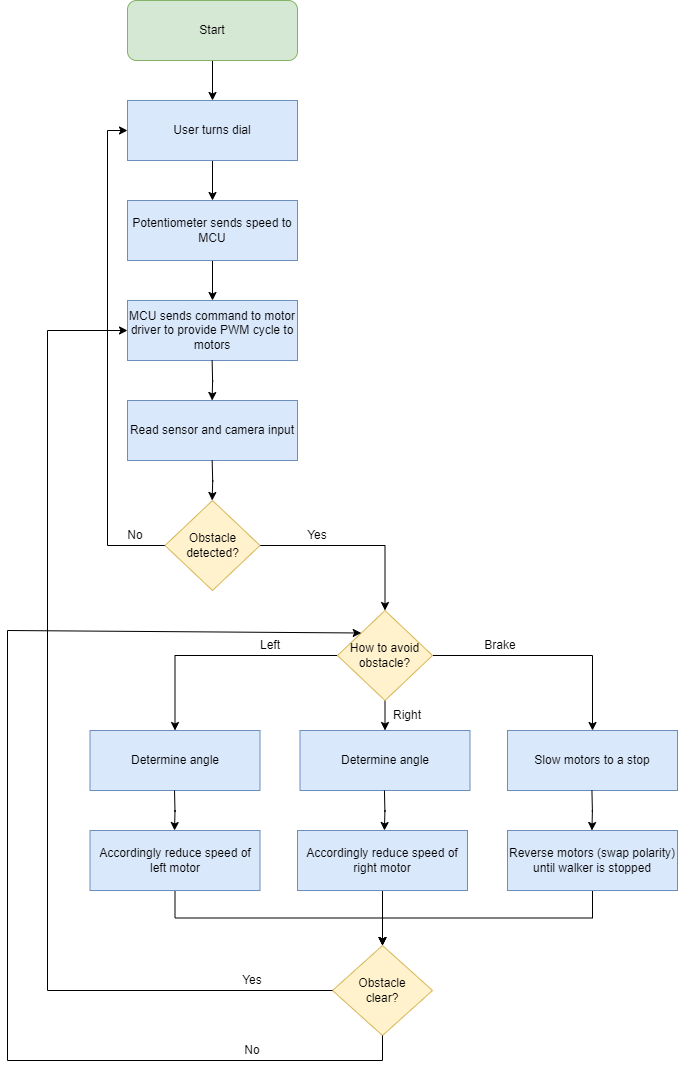
\includegraphics[width=0.7\textwidth]{./Images/motorsw.drawio.png}
	\caption{\label{fig:motorsw}Motor Control Software Diagram}
\end{figure}


\subsubsection{Polite Response to Obstacle in Motion}
\noindent Polite obstacle avoidance is a veering-moded response to moving obstacles, namely people, pets, and vehicles. The inspiration was drawn from real world experiences, where an obstacle will non-intelligently obstruct fluid travel straight ahead. If there is for example, a person walking from left to right (rollator frame of reference) across the camera field of vision, we can track the coordinates of its detection square, and form some abstract calculation of its velocity. We also have some idea of how fast this might be traveling based on other environmental data obtained by the camera; however, methods beyond the scope of this project would likely be required to harness this and improve avoidance strategies. Nevertheless, knowing the direction of travel of the obstacle means FORWARD can veer the user in the opposite direction. Being opposite is paramount because traveling behind the forward path of the obstacle will vastly decrease the chance of collision, and it will not infringe on either party's convenience or safety. The effects of collision for a stationary object are less severe compared to the likes of a running person or God forbid, a car. FORWARD will be able to confidently halt the user from these dangerous situations, and strategically navigate around them in a seamless manner.\\
\begin{figure}[H]
	\centering
	\rotatebox[origin=c]{90}{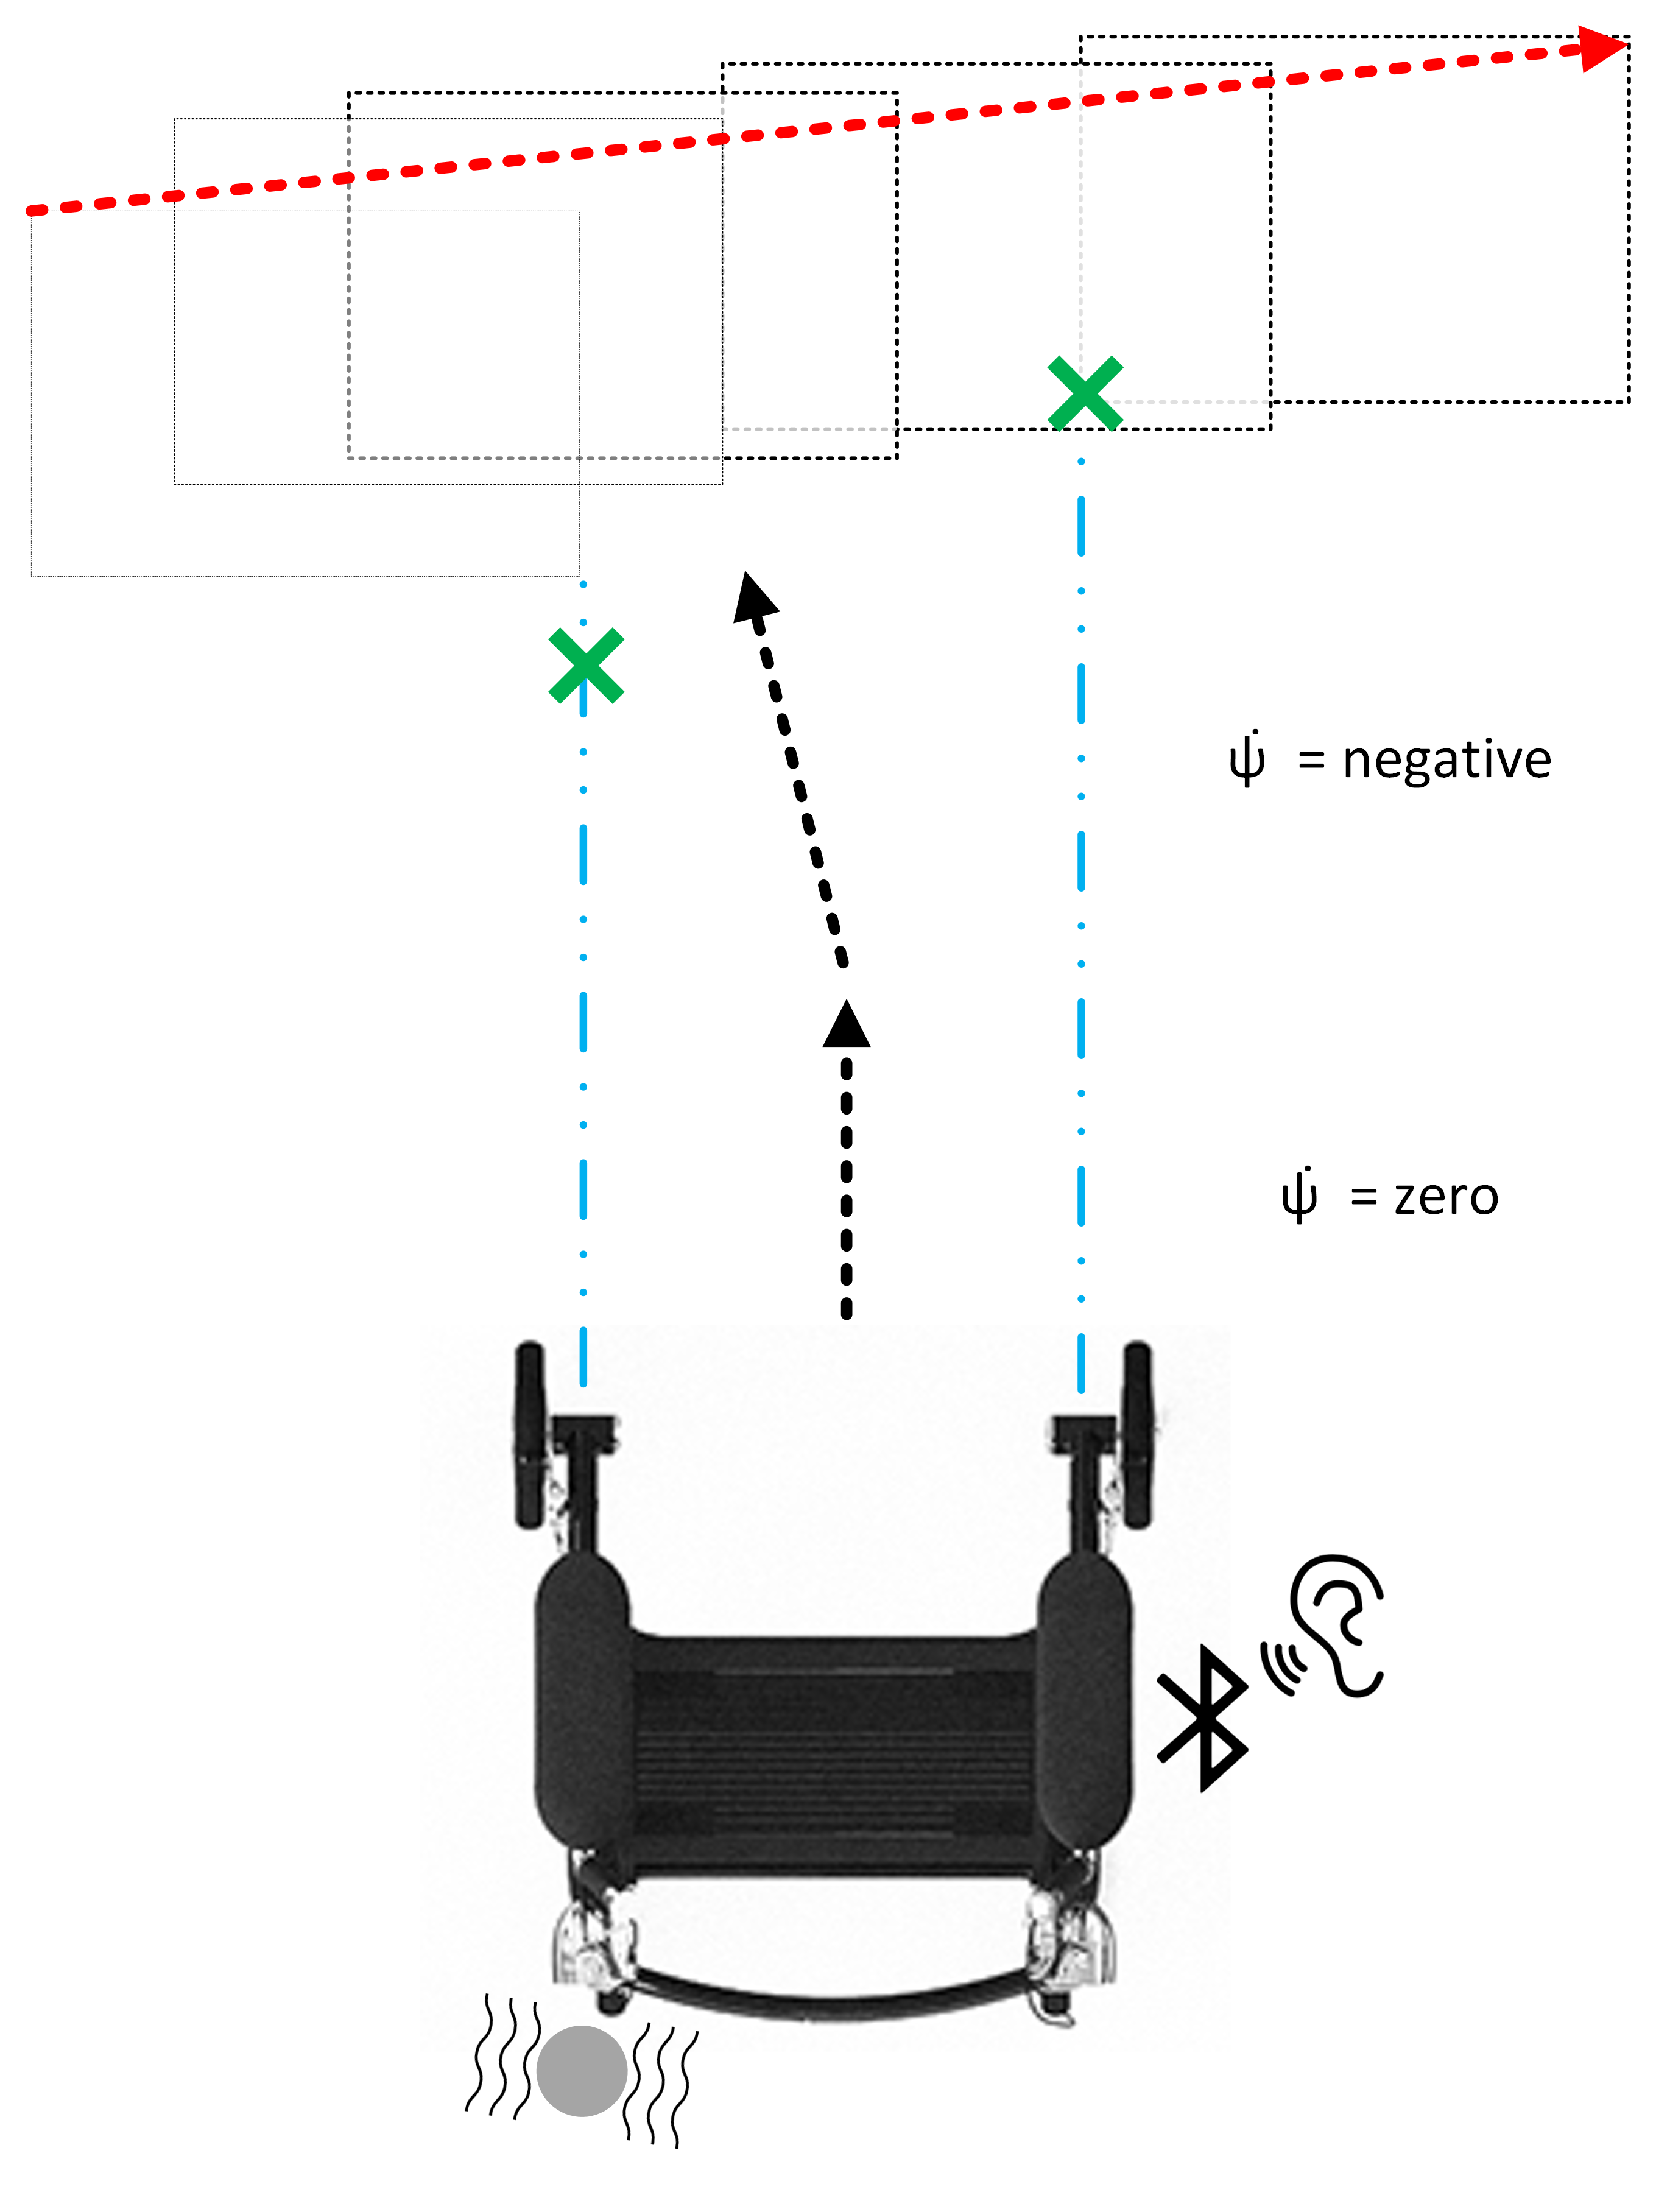
\includegraphics[width=0.6\textwidth]{./Images/Polite-Mobile-Obstacle-Avoidance.png}}
	\caption{\label{fig:polite}Polite Obstacle Avoidance}
\end{figure}
\noindent In figure \ref{fig:polite}, the red dotted line is the assumed constant velocity of an obstacle, represented by the dotted rectangle, crossing from left (S2) to right (S3). An initial deadset detections is made at the lower green X, when the obstacle passes into sensor S2's own field of view. The second green X above indicates the last moment (MCU refresh frame) when the obstacle is considered to be "in the way." After passing by, S3 will return to max range reading, indicating the dormant navigation mode can be re-entered, assuming no other obstacles have come into view. The pulsed blue line is the ultrasonic energy path of transmission and reception. The black dotted line is the direction of the rollator velocity, which is also shown to change to move forward (in the direction of negative a yaw angle), politely behind the moving obstacle. Also pictured is both audio and haptic feedback being activated and actuated.\\

\subsubsection{IMU and Stability}
\noindent In section 6.4.2 on Incline and Decline Stability, we showed that the rollator must not be able to roll backward against the user whilst attempting to climb a slope. In order to accomplish this prevention, the motors must compensate for the incline. When the IMU detects a negative angle, indicating an incline, the MCU will increase the PWM duty cycle driving the motors as a function of the angle. The way we determine how much to increase the speed is dependent on change in force Typically, the force applied as the rollator moves forward is $F_{level}$. On an incline, the rollator must overcome the frictional and weight forces of  $F_{incline} = \mu m g \cos(\theta) + m g \sin(\theta)$, whereas $F_{level}$ would typically only have to overcome $\mu m g$. Thus, $F_{incline} - \mu m g \cos(\theta) + m g \sin(\theta)  = F_{level} - \mu m g$. Ideally, we would be able to use a pressure sensor to measure the exact weight of the user as well as somehow measure the exact coefficient of friction between the wheels and the ground. However, this is outside of our scope, so we will assume a typical sidewalk coefficient of friction of 0.5\cite{osha2003} and a maximum weight of 360lbs (300 from the user and 60 from the walker). The ratio of the speed increase will be calculated to be $F_{incline}/F_{level}$.\\

\subsection{Feedback Protocols}

\subsubsection{Haptic Feedback}
\noindent When an obstacle is initially detected, the motor on the side in which the obstacle is detected will vibrate in pulses until it is time for FORWARD to either steer or brake to avoid the obstacle if needed. If the walker needs to veer to the right or to the left in response to the obstacle, the handlebar in the direction the walker is steering toward will vibrate for the duration of the turn. The ERM motors will vibrate in pulses while the walker is turning, with the period of the pulses dependent on the steering angle. If FORWARD needs to take a sharp turn, the haptics will vibrate more often with shorter pulses, whereas a slight turn will vibrate with longer pulses. If FORWARD is coming to a stop, both haptic motors will vibrate simultaneously until the walker has come to a complete stop. After a short delay, perhaps around five seconds, if the obstacle passes, both of the haptic motors will vibrate twice for around one second per pulse to indicate the walker will move forward again. The motion will begin after this warning is given to the user. If the obstacle does not pass but instead FORWARD needs to turn away from the obstacle after coming to a complete stop, one haptic motor will vibrate twice for around one second per pulse on the side in which the walker is turning toward.\\ 

\noindent Considering the data captured and processed by the camera, we also need a way for the user to distinguish between different obstacles. The system of haptic feedback will accomplish this using pulse width modulation (PWM). PWM is a method of speed control discussed in section 3.2.6 where voltage is applied for a percentage of a period. When the high voltage pulses are wider (the motors are spinning at a faster rate), the haptic motors vibrate louder, whereas a shorter voltage pulse results in weaker vibration. Because a louder vibration draws more attention, a sense of urgency is conveyed. Thus, we will use the speed of vibration to indicate the danger of the approaching obstacle. We will first classify each of our recognized obstacles with a danger level (for example, a vehicle most dangerous, then a human, and grass least dangerous) and set the speed of the motors accordingly.\\

\begin{figure}[H]
	\centering
	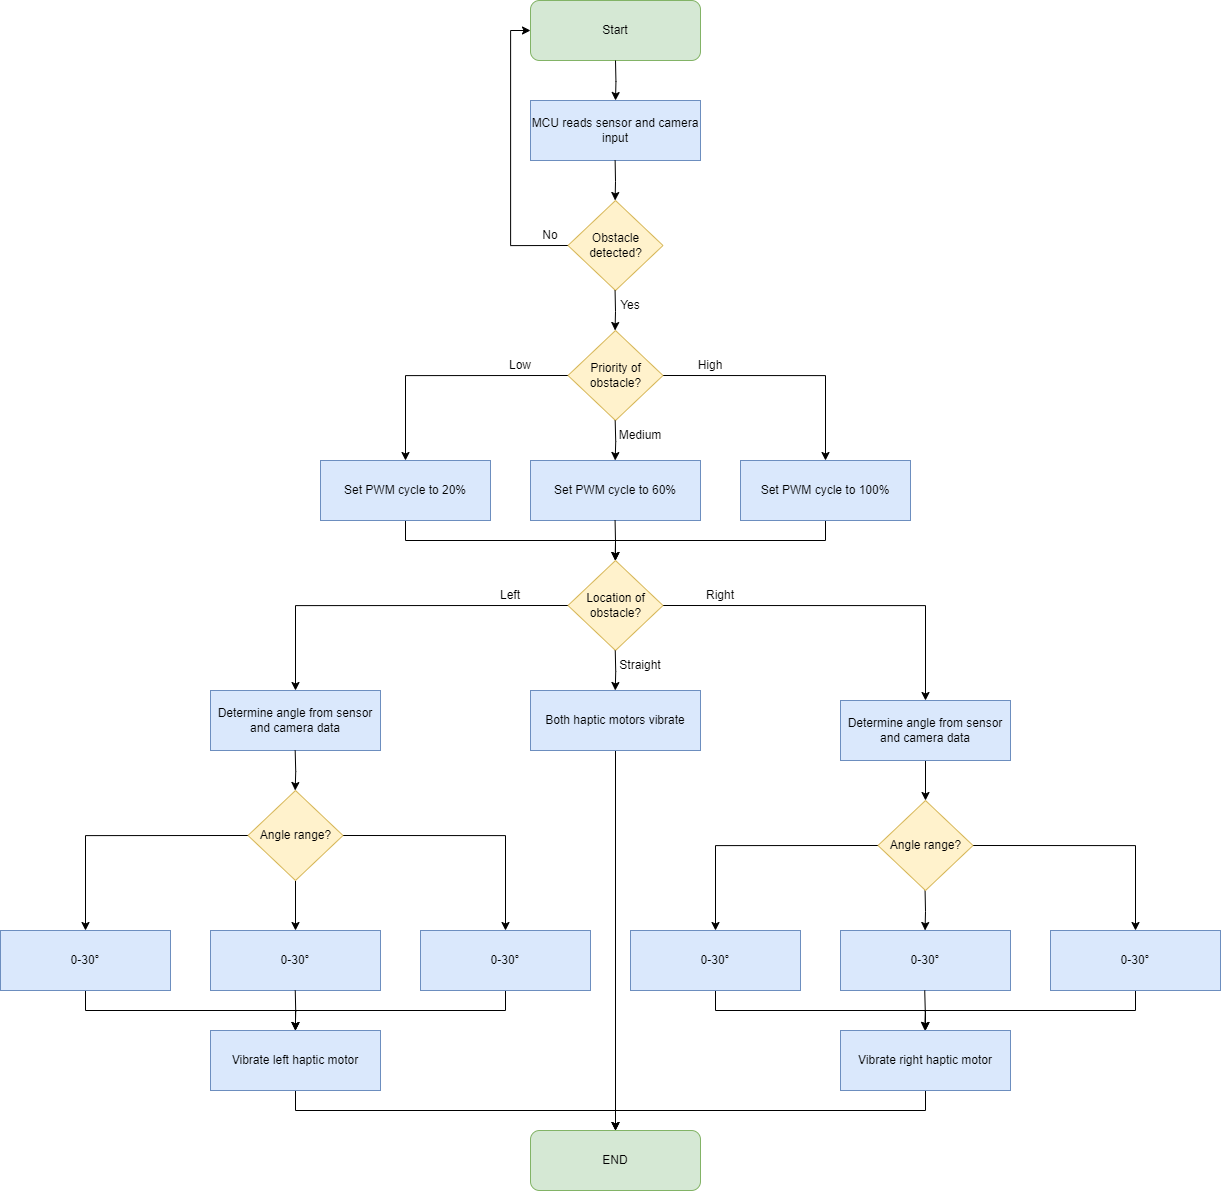
\includegraphics[width=1\textwidth]{./Images/hapticsw.png}
	\caption{\label{fig:hapticsw}Haptic Control Software Diagram}
\end{figure}

\subsubsection{Audio Feedback}

\noindent A crucial aspect to the user's awareness is audio feedback. Once the MCU processes the camera and sensor input, it is able to detect and identify obstacles. Obstacles that come within range of the ultrasonic and LiDAR sensors will also be identified by the camera using computer vision. An audio file will be played through the earbuds that names the obstacle identified. Also, based on the sensor data, the direction FORWARD moves will be relayed to the user through an audio message sent to the earbuds. As an example, if a person if walking toward the user on the right side, the audio playback will be "Person detected. Turning left."\\

\begin{figure}[H]
	\centering
	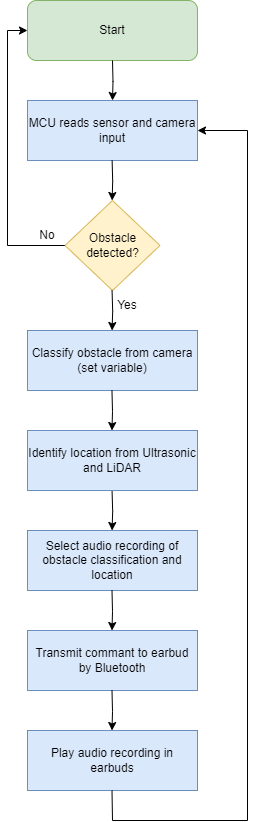
\includegraphics[width=0.25\textwidth]{./Images/audio2.drawio.png}
	\caption{\label{fig:audiosw}Audio Feedback Software Diagram}
\end{figure}

\subsection{Headlight Protocol}
\noindent  Predominantly, the headlight is a safety feature so that the rollator is visible to vehicles and pedestrians at night. The system operating the headlight is quite simple. A photoresistor will be mounted above the headlight detecting the input of light above. When the amount of lumens reduces beyond a certain threshold for a certain duration (i.e. five seconds to ensure the reduction is not a passing shadow), then the headlight will have voltage applied to it. Although not one of our requirements, we may choose to apply a PWM cycle to the headlights to increase the brightness of the headlights as the environment becomes darker, which will save power.\\